% -*- root: ../main.tex -*-
%!TEX root = ../main.tex
% this file is called up by main.tex
% content in this file will be fed into the main document
% vim:textwidth=80 fo=cqt

\clearpage
\chapter{Introduction}\label{ch:intro}

% need a symbol Nomenclature

\capolettera{T}{ightening} emissions  regulations on various  industrial sectors
have led  to a renewed interest  in sustainable energy sources  in recent years.
In  particular,  the  burgeoning  demand  for  clean  energy  has  prompted  the
automotive and  consumer electronics industries  to explore advanced  methods of
energy storage~\cite{Weiss2011}. Li-ion batteries\footnote{The term(s) `cell(s)'
and  `battery(ies)'  are  used  interchangeably  in  this  thesis.  Technically,
an  electrochemical  cell is  the  smallest  self-contained  unit (housed  in  a
packaging  with  terminal  connectors)  that  is capable  of  both  storing  and
delivering energy. A battery  (also referred to as a battery  `pack') is made up
of  a  group  of cells  arranged  in  a  custom  configuration to  meet  certain
system-level  voltage,  current and  power  demands.  The  focal point  of  this
thesis  is  a  single cell  (a  discussion  of  what  this entails  is  provided
shortly  hereafter,  thereby  narrowing  down the  geometrical  scope  of  large
portions  of this  thesis  to  a precisely  defined  unit).  Scaling of  various
quantities from  the pack  level down  to the cell  level is  discussed wherever
appropriate.}  seen as  key enablers  in this  quest due  to the  attractiveness
of  their  high   energy  and  power  densities  compared   to  other  competing
non-conventional energy  storage technologies~\cite{Ibrahim2008}.  However, with
this  surge in  energy  storage  demands comes  stricter  requirements for  cell
longevity,  performance,  and  adhesion  to  safety  requirements,  particularly
for  adoption  in  mainstream  transport  electrification~\cite{Andrea2010}.  In
contrast  to  other  incumbent  technologies,  lithium-ion  cells  have  several
advantages  such  as   high  energy  density,  long   lifecycles,  low  internal
resistance,  low self-discharge,  long  cycle life,  fast  charge and  discharge
cycles~\cite{Reddy2011,Plett2015}\fxnote{Ragone plot here}.  This makes them the
preferred  choice  for storage  and  on-demand  retrieval  of energy  in  modern
consumer electronics and~\glspl{xeV}.

% Different type of cells - Prismatic,  pouch and cylindrical. How pouch cells are
% used in automotive industry acknowledge Tesla, but cite counter citations. Layer
% photos etc

% Precise definition of cell unit
% \section{Geomtery}
% C-rate definition

% Mention  that stuff  is  applicable for  both Lithium  ion  and Lithium  polymer
% chemistries.

\section{Working Principle}\label{subsec:liionchemistry}

This section  provides a  brief overview of  the essential  chemistry principles
that helps to describe the working principle of a lithium ion cell.

In  a Li-ion  cell,  the  positive electrode  consists  of  porous particles  of
Lithium-Transition Metal Oxide (MO)  compounds. The negative electrode typically
employs  some  variant  of  microporous  graphite.  The  porous  nature  of  the
electrodes provide pathways for lithium  ion conduction through the electrolyte.
Due  to  the  special  construction  of the  electrode  structure,  there  exist
interstitial  sites  which act  as  intercalation  spots for  Lithium  shuttling
between the two  electrodes. The electrolyte, whose dynamics are  ignored in the
\gls{spm}, helps  in the  conduction of \ch{Li^+}  ions. The  separator membrane
allows  the passage  of  these ions  between the  two  electrodes, but  prevents
internal  short-circuit  by inhibiting  electronic  conduction  through it.  The
current collectors facilitate  passage of electrons generated  during the charge
transfer reaction  at particle surface  to the  external circuit. With  the help
of \cref{fig:chargetransferprocess}  the  steps  involved  in  this  process  is
detailed next.

\begin{figure}[!htbp]
    \centering
    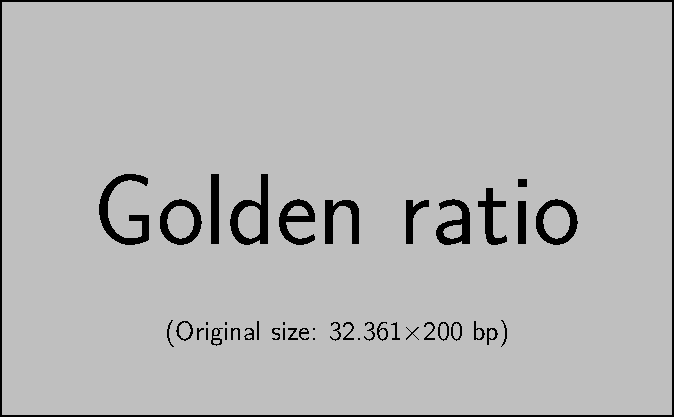
\includegraphics{placeholder_images/example-image-golden.pdf}
    \caption[Charge-transer and basic working mechanism of a Li-ion cell]{Simplified representation of charge-transfer
    process and illustration of basic working mechanism of a Li-ion cell.}
    \label{fig:chargetransferprocess}
\end{figure}

At fully  charged condition,  the majority  of Lithium in  the system  is stored
within  the  negative  electrode  microstructure.  During  discharge,  \ch{Li^0}
atoms  diffuse  out of  deep  interstitial  sites  towards  the surface  of  the
particles  in  the negative  electrode.  At  the surface  (electrode-electrolyte
interface),  a charge-transfer  process takes  place according  to Butler-Volmer
kinetics \cref{eq:butlervolmer}, leading to the  formation of \ch{Li^+} ions and
electrons.  The electrons  are passed  to the  external circuit  through \ch{Cu}
current collectors  onto which  the conductive matrix  composed of  the negative
electrode material and binders is coated.  The \ch{Li^+} ions travel through the
electrolyte phase,  crossing the  separator membrane  to the  positive electrode
where they  encounter an  electron influx  from the  external circuit.  A charge
transfer  reaction  takes  place  at  the  surface  of  the  positive  electrode
particles, leading to the formation of neutral \ch{Li^0} atoms that diffuse into
the positive electrode microstructure.

During  the   charging  process,  the   reverse  phenomena  occur.   Lithium  is
de-intercalated  from  the  positive  electrode and  a  similar  charge-transfer
happens   at   the   surface,   leading    to   the   formation   of   \ch{Li^+}
ions   which   reach   the   negative   electrode   by   passing   through   the
separator.  At   the  surface  of   the  negative  electrode   particles,  these
ions   absorb   electrons   from   the  external   circuit,   leading   to   the
formation   of   neutral   \ch{Li^0}   that  diffuses   into   interior   vacant
spaces  in  the  layered   graphite  electrode.  The  charge-transfer  mechanism
and  sequence   of  events  are   depicted  in \cref{fig:chargetransferprocess}.
\Cref{eq:NegElectrodeRxn,eq:PosElectrodeRxn} summarise the  reactions during the
charging and discharging process at the surfaces of both electrode materials.
\begin{align}
    \ch{Li_{$x$} C                            &<=>[\tiny{discharge}][\tiny{charge}] C + $x$ Li^+ + $x$ e^-}\label{eq:NegElectrodeRxn}\\
    \ch{Li_{1-$x$} M O2 + $x$ Li^+  + $x$ e^- &<=>[\tiny{discharge}][\tiny{charge}] LiMO2}\label{eq:PosElectrodeRxn}
\end{align}
where    \ch{M}   represents    a    transition   metal    compound   such    as
\ch{Ni_{1/3}Co_{1/3}Mn_{1/3}}   (NMC),   \ch{Ni_{0.8}Co_{0.15}Al_{0.05}}   (NCA)
amongst other  choices~\cite{Reddy2011}. Assuming  no loss of  cycleable Lithium
due to  parasitic side  reactions or  through other  mechanisms, the  process is
fully reversible.


The electrochemical potential at each electrode  is dependent upon the extent of
its  lithiation. An  empirical  relationship of  each  electrode's potential  as
a  function  of  its  stoichiometry  can be  obtained,  and  is  dependent  upon
the  specific design  and  material  properties of  each  active material  under
consideration. Finally, the \gls{ocv} of the cell is obtained by subtracting the
negative electrode potential from its positive electrode counterpart.


\section{Battery Modelling}

Through accurate model representations  of the electrochemical-thermal behaviour
of  the cell,  advanced monitoring  and control  strategies can  be deployed  to
tackle  the current  research  topics  in Li-ion  batteries  such as  increasing
cycle-life,  improving  operational   safety  and  performance~\cite{Plett2015}.
Over  the  past two  decades,  efforts  have  been  made to  construct  accurate
models  to  describe  the  physical, electrical,  thermal,  electrochemical  and
system-level performance  of Li-ion  cells, leading  to modelling  strategies of
various  level of  sophistication. For  the  interested reader,  the article  by
Grazioli~\etal~\cite{Grazioli2016a} provides  a broad introduction to  the topic
of computational  modelling of  lithium ion batteries.  Large in-roads  into the
depth of the modelling  art can be made by perusing  comprehensive books on this
topic such  as those by  Plett~\cite{Plett2015}, Hariharan~\cite{Hariharan2017},
and Rahn and Wang~\cite{Rahn2013}.

The  need  to  address  the  operational challenges  of  lithium  ion  batteries
in   an   embedded   environment   such  as   on-board   an   electric   vehicle
has   led   to  an   increased   impetus   on   the  development   of   advanced
\glspl{bms}~\cite{Bergveld2002}. In vehicular  applications, the only measurable
quantities  of  a  lithium  ion  cell are  its  terminal  voltage,  current  and
temperature. This implies  that several internal states of the  cell such as its
\gls{soc}, whose  real-time computation is  vital to the optimal  performance of
the cell, need to be estimated from these available measurements. Therefore, the
performance  of  a \gls{bms}  for  tasks  such  as  online state  estimation  is
dependent upon  the fidelity  of the underlying  cell model  used. Sophisticated
models of the  cell enable these quantities to be  estimated more accurately and
facilitate the implementation  of advanced control algorithms.  Therefore, it is
imperative  that  the cell  model  used  is suitable  for  being  embedded in  a
real-time \gls{bms}.

Most battery  models have the primary  goal of accurately predicting  the cell's
terminal  voltage  at each  time-step.  This  is so  that  the  output from  the
predictor routine  can be compared  to the  measured voltage and  the difference
between them  may be used in  a suitable corrector-subroutine to  improve future
prediction.  The combined  information from  the model  and measurement  is then
blended in a suitable way to estimate the cell's \gls{soc}.

More   advanced  models   strive   to  provide   insight   into  various   other
physico-chemical quantities  that could  affect the health  of the  battery. The
field of  Li-ion battery modelling can  be classified into two  broad categories
---
\begin{enumerate*}[label=\roman*)]
    \item empirical/ad-hoc \glspl{ecm}, and
    \item detailed  \glspl{pbm} that are based  upon first principles.
\end{enumerate*}
A  comprehensive summary  of  various models  that  belong to  each  of the  two
categories  is  discussed  in Seaman~\etal~\cite{Seaman2014}.  A  characteristic
aspect that contrasts  them is the fact that these  two approaches are typically
at loggerheads with each other in terms of their computational complexity.

\subsection{\glsfmtlong{ecm}s}\label{subsec:ecms}

\glspl{ecm}  employ circuit  elements  such as  voltage  sources, resistors  and
capacitors to  model the behaviour  of batteries at their  electrical terminals.
The cell's  thermal subsystem may  also be  modelled by an  analogous electrical
circuit. The  parameters of the  circuit are  typically functions of  the cell's
current, \gls{soc} and  temperature and can be implemented as  a lookup table by
curve-fitting  the model  to experimental  data. Using  such equivalent  circuit
models, two simple methods are available to compute the cell's \gls{soc} ---
\begin{enumerate*}[label=\itshape\alph*\upshape)]
    \item manufacturer-supplied  lookup table or graph of \gls{ocv} versus \gls{soc}, and
    \item numerically integrating the charge passed in and out of the cell over time, commonly referred to as coulomb counting.
\end{enumerate*}
Both methods are computationally  amenable for small-scale embedded applications
like  consumer  electronics;  however,  neither  one is  robust  to  handle  the
stringent demands in performance imposed  by modern vehicular applications.

Advanced state estimation algorithms such  as nonlinear Kalman filters may still
be able to use \glspl{ecm} as the plant model and obtain reasonable estimates of
the  cell's  \gls{soc}~\cite{Plett2006,  Sun2011}. However,  the  usefulness  of
\glspl{ecm} is limited by the fact that their parameters are derived essentially
by a  curve-fitting process using a  standard set of training  data. Since these
models are  not based on  any physical phenomena,  their ability to  predict the
cell's general behaviour  is extremely poor especially when  subjects to current
profiles well  outside their training  realm. Another important  disadvantage of
equivalent circuit  models is that they  do not allow insights  into the various
internal states of the cell.

\glspl{ecm}  of  lithium  ion  batteries   have  been  extensively  studied  and
are  widely  applied.  However,  the aforementioned  difficulties  render  their
reliability and  accuracy questionable,  especially under highly  demanding load
profiles  experienced by  the battery  packs in  \glspl{xeV}. The  boundaries of
their  performance have  been well-quantified  (see~\cite{Plett2015,Plett2016}).
Although  various estimation  and control  algorithms continue  to be  developed
around them, the  \glspl{ecm} themselves are no longer the  subject of extensive
research. Hence, this thesis does not discuss them further.

\subsection{\glsfmtlong{pbm}s}\label{subsec:pbms}

\glsreset{pbm}

\glspl{pbm} consist of  governing equations that construct a  realization of the
behaviour of the cell based  upon electrochemical principles such as equilibrium
thermodynamics,  material  diffusion  and  reaction  kinetics.  The  fundamental
advantage  to this  modelling approach  is that  it is  possible to  compute the
evolution of  internal states of  the cell  for arbitrary current  profiles. The
difficulty with  the physics-based  modelling approach  lies with  obtaining the
values  of all  the physical,  geometric, electrochemical,  thermal and  kinetic
parameters  of the  cell. Usually,  these parameters  are closely  guarded trade
secrets by cell cell manufacturers.

In  some  cases, it  may  be  possible to  obtain  a  subset of  these  physical
parameters  can be  obtained  by dissection  of cells  in  an inert  environment
followed  by further  characterisation  through specialised  lab equipment.  For
instance, Ecker~\etal~\cite{Ecker2015} demonstrate  the reverse-engineering of a
\SI{7.5}{\amphour} pouch cell by Kokam  Ltd.\ to obtain its physical parameters.
Nevertheless, this is a tedious process and is feasible only with access to such
specialised lab  equipment. Furthermore, the  results from these  experiments is
susceptible to characterisation errors as well as cell-to-cell variations due to
production spread. Therefore, some form of system identification method needs to
be employed  for estimating the rest  of the physical parameters  required for a
\gls{pbm}.  Furthermore, it  is  a common  practice to  rely  on published  data
for  the values  of  certain cell  parameters  that do  not  depend on  physical
construction, especially for those that remain universally true for a particular
li-ion chemistry.

The challenges involved  in model parametrisation is a research  exercise of its
own merit and  is not addressed in  this thesis. A redeeming factor  is that the
task of  parametrisation is a  one-off problem that  appears early in  the model
deployment  stage,  after which  the  rewards  of  superior performance  of  the
\glspl{pbm} can be reaped. Once  the model parameters are available, \glspl{pbm}
can be used in  aiding a deeper understanding of the working of  the cell and in
answering research  questions that could  otherwise not be answered  with simple
\glspl{ecm}. One area  of focus of this  thesis is to broach  a less-probed area
--- exploring  the possibility  of using  a \gls{pbm}  for the  \emph{design} of
pouch cells used in automotive applications. The author's findings on this topic
shall be presented in \cref{ch:modelbaseddesign}.

A major disadvantage of \glspl{pbm} from an implementation point of view is that
solving for  the model's field  variables is time-consuming. In  particular, the
more  sophisticated  \glspl{pbm}  require  the use  of  multi-physics  \gls{pde}
solvers  and  hence  are  not  typically  suitable  for  embedded  applications.
Nevertheless,  for   high  performance   applications  such  as   in  automotive
\glspl{bms}  wherein   state-of-health  monitoring  is  crucial,   there  is  an
overwhelming  demand for  obtaining insight  into internal  cell variables.  For
instance, the real-time computation of surface concentration of \ch{Li^0} in the
solid particles enable  the \gls{bms} to avoid regulate power  flow into and out
of the cell to proactively avoid plating and degradation of the cell.

In view of this consideration, model  order reduction techniques are seen as key
enablers that facilitate in porting the first-principles based predictive powers
of \glspl{pbm}  into a  real-time microcontroller.  This thesis  shall therefore
have  a  strong  focus  on  both the  analysis  and  implementation  aspects  of
\glspl{rom}.

\section{The \glsfmtlong{dfn} model}

Doyle,  Fuller and  Newman~\cite{Doyle1993,Fuller1994}  developed an  isothermal
physics-based  porous electrode  model of  the  cell capable  of describing  its
internal variables such as
\begin{enumerate*}[label=\itshape\alph*\upshape)]
    \item potential on the solid particles,
    \item potential in the electrolyte solution,
    \item concentration of \ch{Li^0} in the solid particles,
    \item ionic concentration in the electrolyte solution, and
    \item molar flux density of lithium at the solid-electrolyte boundary.
\end{enumerate*}
The most popular computational implementation  of the \gls{dfn} equations is the
\gls{p2d} model.  In the  \gls{p2d} implementation, all  field variables  of the
\gls{dfn} model are  computed at each spatial location location  along the axial
thickness of the  cell. However, the solid concentration  in spherical electrode
particles is solved in a radial  co-ordinate system that is perpendicular to the
axial direction. The axial and radial  dimensions are coupled at each particle's
surface through  the molar flux  density describing  the rate of  pore-wall flux
that  crosses from  solid  into  electrolyte or  vice-versa.  The equations  and
boundary conditions for  the \gls{p2d} implementation of the  \gls{dfn} model is
shown in \cref{tbl:dfneqns}.

% -*- root: ../main.tex -*-
%!TEX root = ../main.tex
% this file is called up by main.tex
% content in this file will be fed into the main document
% vim:nospell textwidth=180 foldlevelstart=3 foldlevel=3

% \begin{table}[!htbp]
    \begin{table}[p]
        \centering
        \caption[]{}
        % \label{tbl:charSimspmp2d}
        \begin{threeparttable}
            \begingroup
            \makeatletter\def\f@size{10.0625}\check@mathfonts
            % \addtolength{\jot}{0.75em}
            \addtolength{\jot}{0.875em}
            \begin{tabular*}{\textwidth}{@{} l c r l r @{}}
                \toprule
                Region & Governing equations & \multicolumn{3}{c}{Boundary conditions} \\
                \midrule
                \multicolumn{1}{l |}{\rotatebox[origin=c]{+90}{\makecell{\small Electrodes \\ \small \linnegpos}}} &
                $\begin{aligned} % placement: default is "center", options are "top" and "bottom"
                    \vphantom{\diffp{c_\slsub}{r}{\mathrlap{r = R_\pl}}}
                    \diffp{c_\slsub}{t} &= \frac{D_\slsub}{r^2}\diffp{}{r}\left(r^2 \diffp{c_\slsub}{r} \right) \\
                    \vphantom{\diffp{c_\text{e}}{x}{\mathrlap{x = l_\text{tot}}}}
                    \varepsilon_l \diffp{c_\text{e}}{t} &= \diffp{}{x}\left(D_\effl
                    \diffp{c_\text{e}}{x} \right) + (1 - t^0_\text{+}) a_\slsub j_l \\
                    \vphantom{\diffp{\phi_\text{e}}{x}{\mathrlap{x = 0}}} 0 &= \diffp{}{x}\left(\kappa_\effl \diffp{\phi_\text{e}}{x}\right) + \diffp{}{x}\left(\kappa_\effl \frac{2 R T(t)}{F} (t^0_{+}-1)\diffp{ \ln c_\text{e}}{x}\right) \\
                    \vphantom{\sigma_\effl\!\diffp{\phi_\slsub}{x}{\mathrlap{\substack{\vphantom{\displaystyle M}x = x_\text{pos/sep}\\x = x_\text{neg/sep}}}}} a_\slsub F j_l &= \diffp{}{x}\left(\sigma_\effl \diffp{\phi_\slsub}{x}\right) \\
                    % j_l &= k_\lr c^\alpha_\text{e}\left(c_\slmax - c_\slsurf\right)^\alpha c^\alpha_\slsurf\left( \exp\left(\frac{\left(1-\alpha\right)F}{R T}\eta\right) - \exp\left(-\frac{\alpha F}{R T}\eta\right) \right)
                    j_l &= 2 k_\lr \sqrt{c_\text{e}\left(c_\slmax - c_\slsurf\right) c_\slsurf} \sinh \left(\frac{0.5 F}{R T(t)} \eta_l \right)
                \end{aligned}$ &
                $\begin{aligned}
                    \vphantom{\diffp{c_\slsub}{r}{\mathrlap{r = R_\pl}}} \diffp{c_\slsub}{r}{\mathrlap{r = 0}}\hspace{1mm} &= 0, \\
                    \vphantom{\diffp{c_\text{e}}{x}{\mathrlap{x = l_\text{tot}}}} \diffp{c_\text{e}}{x}{\mathrlap{x = 0}}\hspace{1mm} &= 0, \\
                    \diffp{\phi_\text{e}}{x}{\mathrlap{x = 0}}\hspace{1mm} &= 0, \\
                    \sigma_\effl\!\diffp{\phi_\slsub}{x}{\mathrlap{\substack{\vphantom{\displaystyle M}x = x_\text{pos/sep}\\x = x_\text{neg/sep}}}}\hspace{1mm} &= 0, \\
                    % {}&\textemdash{}{}
                    {}&\xdash[1.25em]{}
                \end{aligned}$ &
                $\begin{aligned}
                    \diffp{c_\slsub}{r}{\mathrlap{r = R_\pl}}\hspace{1mm} &= \frac{-j_l}{D_\slsub} \\
                    \diffp{c_\text{e}}{x}{\mathrlap{x = l_\text{tot}}}\hspace{1mm} &= 0 \\
                \vphantom{\diffp{\phi_\text{e}}{x}{\mathrlap{x = 0}}} \phi_\text{e}\Bigr\rvert_{\mathrlap{x=l_\text{tot}}} \hspace{1mm}&= 0 \\
                % \sigma_\effl\!\diffp{\phi_\slsub}{x}{\mathrlap{\subalign{x&=0\\x&=x_\text{tot}}}} &= \frac{-I}{A} \\
                \vphantom{\sigma_\effl\!\diffp{\phi_\slsub}{x}{\mathrlap{\substack{\vphantom{\displaystyle M}x = x_\text{pos/sep}\\x = x_\text{neg/sep}}}}} \sigma_\effl\!\diffp{\phi_\slsub}{x}{\mathrlap{\substack{\!\!\!\!\!x=0\\x=x_\text{tot}}}}\hspace{1mm} &= \frac{-I}{A} \\
                % \sigma_\effl\!\diffp{\phi_\slsub}{x}{\mathrlap{\substack{\begin{mysubarray} x &=0 \\ x &=x_\text{tot}\end{mysubarray}}}} &= \frac{-I}{A} \\
                % {}&\textemdash{}{}
                {}&\xdash[1.25em]{}
            \end{aligned}$ &
            $\begin{aligned}
                \vphantom{\diffp{c_\slsub}{r}{\mathrlap{r = R_\pl}}}\refstepcounter{equation}(\theequation)\label{eq:dfnsoliddiff} \\
                \vphantom{\diffp{c_\text{e}}{x}{\mathrlap{x = l_\text{tot}}}} \refstepcounter{equation}(\theequation)\label{eq:dfnliquiddiff} \\
                \vphantom{\diffp{\phi_\text{e}}{x}{\mathrlap{x = 0}}} \refstepcounter{equation}(\theequation) \\
                \vphantom{\sigma_\effl\!\diffp{\phi_\slsub}{x}{\mathrlap{\substack{\vphantom{\displaystyle M}x = x_\text{pos/sep}\\x = x_\text{neg/sep}}}}} \refstepcounter{equation}(\theequation) \\
                \vphantom{\left(\frac{0.5 F}{R T(t)} \eta \right)} \refstepcounter{equation}(\theequation)
            \end{aligned}$ \\
            \bottomrule
        \end{tabular*}
        \endgroup
        \begin{minipage}{\textwidth}
            \bigskip
            \begin{flushleft}
                \raggedright
                \makeatletter\def\f@size{14}\check@mathfonts
                $\begin{alignedat}{2}
                    & \text{\textbullet{} } c_\text{e} &  & \coloneqq c_\text{e}(x,t), \quad  \{x \in [0,l_\text{tot}],\, (x=0)\symbol{"2259} \text{\footnotesize pos/Alcc},\, (x=l_\text{tot})\symbol{"2259} \text{\footnotesize neg/Cucc}\}  \tnote{\dagger}                                                                                                                                                                  \\
                    & \text{\textbullet{} } \phi_\text{e} &  & \coloneqq \phi_\text{e}(x,t)\\
                \end{alignedat}$
                \\[0.5em]
                \fbox{\raggedright \small  \linnegpos}
                $\begin{alignedat}{2}
                    % & \mathbf{\textbf \linnegpos} & {} \\
                    & \text{\textbullet{} } c_\slsub   &  & \coloneqq c_\slsub(r,t), \quad  \{r \in [0,R_\pl],\, (r=0)\symbol{"2259} \text{\footnotesize  particle center},\, (r=R_\pl)\symbol{"2259} \text{\footnotesize particle surface}\}              \\
                    & \text{\textbullet{} } c_\slsurf &  & \coloneqq c_\slsub(r=R_\pl,t)\\
                    & \text{\textbullet{} } \phi_\slsub &  & \coloneqq \phi_\slsub(x,t)\\
                    & \text{\textbullet{} } j_l          &  & \coloneqq j_l(x,t) \\
                    & \text{\textbullet{} } \sigma_\effl &  & = \sigma_l \cdot \varepsilon_l \\
                    & \text{\textbullet{} } \eta_l        &  & \coloneqq \eta_l(x,t) = \phi_\slsub(x,t) - \phi_\text{e}(x,t) - \mathcal{U}_l(c_\slsurf) \\[0.5em]
                \end{alignedat}$
                % \medskip
                \fbox{\raggedright \small  \linnegseppos}\\[0.5ex]
                $\begin{alignedat}{2}
                    & \text{\textbullet{} } D_\effl    &  & = D \cdot \varepsilon_l^{\text{brugg}_l}                                                                                                                                                  \\
                    & \text{\textbullet{} } \kappa_\effl &  & = \kappa \cdot \varepsilon_l^{\text{brugg}_l} \\
                    & \text{\textbullet{} } D        &  & \coloneqq D(c_\text{e},T) = 10^{-4} \times 10^{-4.43 - \frac{54}{T(t) - 229 - 5\times10^{-3} c_\text{e}(x,t)} - 0.22\times10^{-3} c_\text{e}(x,t)}               \\
                \end{alignedat}$
                \\
                \makeatletter\def\f@size{14}\check@mathfonts
                $\begin{alignedat}{2}
                    & \text{\textbullet{} }  \kappa   \: \quad&  & \coloneqq \kappa(c_\text{e},T)\, = \parbox[t]{11.60cm}{\raggedright $\scriptstyle 10^{-4} \times c_\text{e}(x,t)\Big(-10.5 + 0.668\times10^{-3} c_\text{e}(x,t) + 0.494\times10^{-6} c_\text{e}^2(x,t) + \big(0.074 - 1.78\times10^{-5}c_\text{e}(x,t) - 8.86\times10^{-10}c_\text{e}^2(x,t)\big)T(t) + \big(-6.96\times10^{-5} + 2.8\times10^{-8} c_\text{e}(x,t)\big)T^2(t)\Big)^2$}\\
                \end{alignedat}$
            \end{flushleft}
        \end{minipage}
        \bigskip
        \footnoterule{}
        \begin{tablenotes}
        \item[\dagger] \footnotesize{This definition of the global axial domain $x$, spanning the cell thickness applies for all variables dependent on axial spatial position. Hence the domain definition for $x$ is not repeated elsewhere for the sake of brevity.}
        \end{tablenotes}
    \end{threeparttable}
\end{table}



In  this  thesis,  this  \gls{p2d}  implementation of  the  \gls{dfn}  model  is
considered as  the reference (and  only) \gls{pbm}. Although  thermal dependence
of  parameters  such  as  electrolyte  conductivity  and  diffusivity  is  shown
in \cref{tbl:dfneqns}, a sophisticated description  of detailed thermal dynamics
\ie{} a description  of spatio-temporal evolution of cell's  temperature using a
set of ordinary/partial  differential equations is not considered  in this work.

For those aspects of this thesis dealing with the analysis and implementation of
various  \glspl{rom} and  the  improvements  imparted herein  to  them, only  an
\emph{isothermal}  implementation  (at  \SI{298.15}{\kelvin}) of  the  \gls{p2d}
equations  is  considered.  The  performance  of  the  various  \glspl{rom}  are
compared  against this  reference benchmark.  In consideration  of the  relative
sparsity of  such detailed analysis  of \glspl{rom} in existing  literature (see
\cref{ch:littreview}),  the  author  of  this  thesis  considers  that  such  an
analysis, albeit isothermal, is  the need of the hour and  is imperative to gain
a  deeper  understanding  of  the  performance  boundaries  of  various  popular
\glspl{rom}.  Further  extensions to  the  analysis  presented here  to  include
various thermal effects can be considered for future research.

Since temperature  plays a crucial  role in the  operation of cells  and battery
packs in \glspl{xeV},  an isothermal model is unsuitable for  design purposes. A
model-based design that does not consider thermal effects is likely to stray far
from the operating regimen and fail  spectacularly. Hence, it is not suitable to
use an  isothermal cell model  for informing the design  of cells. On  the other
hand, considering a  sophisticated thermally coupled model is  unlikely to yield
significant gains. Firstly, running  fully coupled electrochemical-thermal model
based simulations  over the  entire design  space is  computationally expensive.
Secondly,  the design  results of  the model  have to  be anyway  verified using
a  reasonable  number of  experimental  prototypes.  Taking into  account  these
considerations it is deemed that, for the design aspect of this thesis, a lumped
thermal model suffices. This simplified thermal model is bidirectionally coupled
to the \gls{p2d} equations (see \cref{tbl:dfneqns}) of the electrochemical model
and  is used  as the  \gls{pbm}  underpinning the  model-based design  discussed
in \cref{ch:modelbaseddesign}.

% need a symbol Nomenclature

% \subsection{Organisation of Thesis}

% nice figure here (with Bohr model of atom)
% \Cref{ch:improveddra} analyses a critical weakness in a sophisticated \gls{rom}
% and proposes a numerical method to circumvent it.
% different \glspl{rom} shall be performed in

% \cite{Seaman2014} provide a comprehensive survey  of the wide range of battery
% models out there.

% This  thesis  strives to  represent  all  physical  quantities in  the  standard
% International  System  of Units  (SI-Units).  However,  there are  some  notable
% exceptions \eg{} for the capacity of a  Li-ion cell, which is represented in the
% practical units  of Ampere  hours (\SI{}Ah),  rather than the  base SI  Units of
% Coulombs (\SI{}{\coulomb}).  Such exceptions  are made  taking into  account the
% prevalent conventions in standard literature.

% \fxnote{Where does  this paragraph go? End  of this section/end of  chapter or
% even  last  chapter?}  The  identification of  individual  parameters  of  the
% \gls{dfn} model  remains a  key area  in battery  modelling that  remains only
% partially  explored. Nevertheless,  this effort  is critical  to ensure  rapid
% adoption  of any  physics-based  model and  sophisticated control  algorithms.
% The  state of  the  art in  this  area, the  challenges  involved and  current
% efforts  in  this  direction are  explored  in \cref{ch:futurework}.  Although
% sensitivity  analysis  of  the  \gls{dfn} parameters  has  been  performed  in
% literature, \fxnote{citation here} the extent to which parameter uncertainties
% influence  the   numerical  values  in  the   $A,  B,  C$  and   $D$  matrices
% of \cref{eq:LTIstatespace} has not yet been attempted. In continuation of this
% research aspect, the order of magnitude  shift in eigen/singular values of the
% relevant system matrix also need to be quantified to enable an informed choice
% about stability of such models for real-time implementations.

% need a symbol Nomenclature
